\section{Fine-tuning of the model}
\subsection{Initial tuning}

\begin{frame}{Batch Normalization, Dropout layers, activation function and pooling}
\begin{itemize}
\item Batch normalization to speed up the training \cite{BatchNorm2015}
\item Initial activation function: $\mathrm{ReLu}: \mathbb{R} \to \mathbb{R}_0^+, x \mapsto \max\{0,x\}$, still MSE of over 15 on the testing 
set, less then 2 on the training set\\
$\Rightarrow$ Overfitting problems
\item Dropout layers \cite{Dropout2014} to make the model more robust and reduce overfitting
%build in one with dropout probability $p=0.5$
\item Solve problems of dead neurons using
\begin{align*}
\mathrm{leakyReLU} : \mathbb{R} \to \mathbb{R}, x \mapsto \begin{cases}
x, x \geq 0\\
c \cdot x, x <0
\end{cases}
\end{align*}
with $c = 0.01$, MSE of around 11 on the testing set and less than 3 on the training set
\end{itemize}
\end{frame}
\subsection{Problems and possible solutions}
\begin{frame}{Problems}
We identified three possible problems for our poor results
\begin{enumerate}
\item Too complex model, as initially used for autonomous driving or insufficient amount of information put into the model
\item Brightnesses/illumination changes in the frames, therefore unstable calculations of the optical flow
\item Too ambiguous splitting, as the training and testing datasets represent totally different road traffic scenarios
\end{enumerate}
\end{frame}

\begin{frame}{Possible solutions}
\begin{enumerate}
\item \textbf{Simplify model}: pooling layers (maximum and average pooling) to get more compression\\
\textbf{Siamese approach}: put flow field and raw frame into the model or put two consecutive frames into the model
\item \textbf{Add additional noise}: add noise before computing the optical flow filed, to get more invariance regarding illumination changes
\item \textbf{Different splitting}: get better ratio between different scenarios, by using a splitting based on the different road traffic situations in the video
\end{enumerate}
\end{frame}

\begin{comment}
\begin{frame}{New splitting: situational splitting}
\begin{figure}
\centering
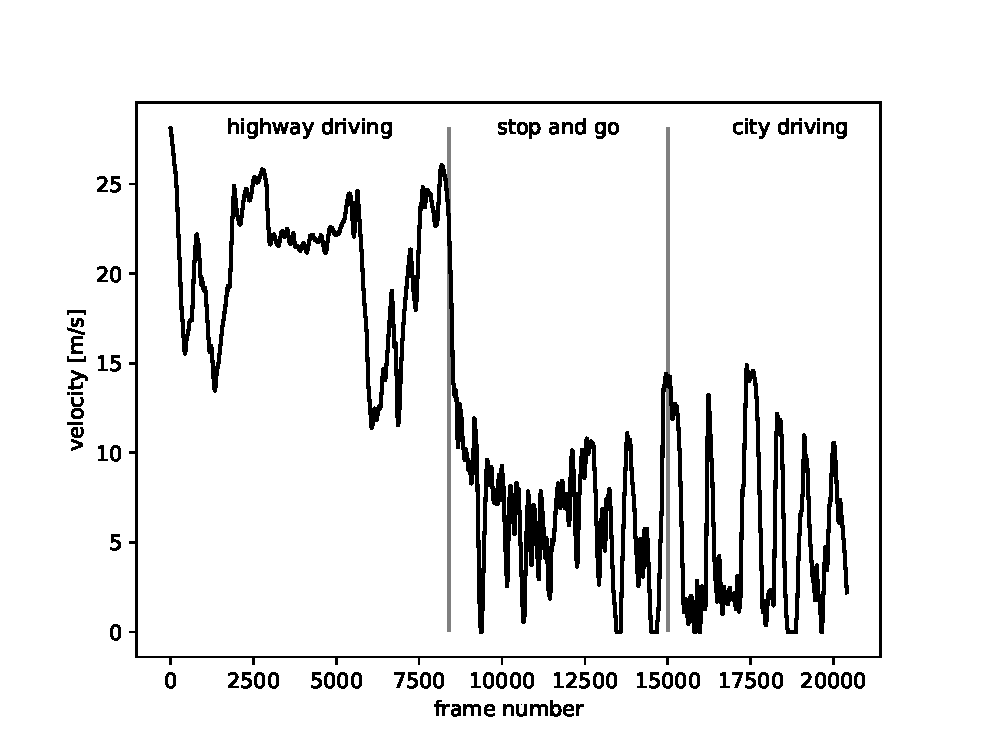
\includegraphics[scale=0.5]{./imgs/plot_speed_time_new_splitting.eps}
\caption{Velocity distribution in the training video, including labels for different scenarios.}
\end{figure}
\end{frame}
\end{comment}

\subsection{Simplified model}
\begin{frame}{Pooling layers (initial splitting)}
\begin{table}[!t]
\normalsize
\centering
\begin{tabular}{lcccc}
\toprule
\multirow{2}{*}{Initial splitting, 8 epochs}  & \multicolumn{2}{c}{$\mathrm{ReLU}$} & \multicolumn{2}{c}{$\mathrm{leakyReLU}$} \\
 & Train & Test & Train & Test\\
\midrule
No pooling & 2.85 & 12.08 & 2.45 & 10.75 \\
Max pooling & 5.62 & 11.82 & 5.52 & 10.29 \\
Max pooling (15 epochs) & - & - & \textbf{3.22} & \textbf{9.63} \\
Average pooling & 7.70 & 11.40 & 6.08 & 13.09\\
\bottomrule
\end{tabular}
\caption{MSE results of the network using different pooling strategies, one dropout layer, two different activation functions and 
the initial splitting. We trained each of the models for eight epochs.}
\end{table}
\end{frame}
\subsection{Siamese approach: flow field and frame (new splitting)}
\begin{frame}{Siamese approach (new splitting)}
RESULTS ARE NEEDED :)\\
Demo videos of highway and city driving scenes under ../demos/
\end{frame}
